\documentclass[aspectratio=169,10pt]{beamer}

% ============================================================
% LASNPA 2026 -- 15th Latin American Symposium on Nuclear Physics
% and Applications, IPEN, Sao Paulo, 7-10 December 2026
% Track: Relativistic Heavy Ions
%
% Oral contribution, 15 min, "Relativistic heavy ion collisions"
% Title as registered in the conference programme (do not change):
%   The Effect of Correlated Experimental Uncertainties on Bayesian
%   Inference of Quark-Gluon Plasma Properties
% Authors: T. S. Domingues, N. Moraes, M. Luzum
%
% Scope (plan of 11 Nov): effect of assumed correlation models on the
% posteriors (compound symmetry, RBF) + scaled-spectra case study +
% first data-driven estimate (GP on HEPData) + outlook.
%
% Figures: \plotorph{file}{width}{height}{text} includes Figures/<file>
% if it exists, otherwise draws a dashed placeholder with the file name.
% Compile twice (metropolis progress bar needs the .nav file).
% ============================================================

\usetheme[progressbar=frametitle, numbering=fraction]{metropolis}
\usepackage[T1]{fontenc}
\usepackage{graphicx}
\usepackage{amsmath,amssymb}
\usepackage{booktabs}
\usepackage{tikz}
\usepackage{pgfplots}
\usepackage{xcolor}
\usepackage{hyperref}
\usepackage{appendixnumberbeamer}
\usetikzlibrary{positioning,arrows.meta,calc,shapes.geometric}
\usepgfplotslibrary{fillbetween}
\pgfplotsset{compat=1.18}

\definecolor{qcdRed}{HTML}{C0392B}
\definecolor{qcdBlue}{HTML}{2980B9}
\definecolor{qcdGreen}{HTML}{1A7A1A}
\definecolor{qcdOrange}{HTML}{D68910}
\definecolor{qcdGray}{HTML}{BDC3C7}
\setbeamercolor{frametitle}{bg=qcdRed,fg=white}
\setbeamercolor{progress bar}{fg=qcdBlue}
\setbeamercolor{alerted text}{fg=qcdBlue}
\setbeamercolor{block title}{bg=qcdBlue!12,fg=black}
\setbeamercolor{block body}{bg=qcdBlue!4,fg=black}
\setbeamertemplate{caption}{\raggedright\insertcaption\par}
\setbeamertemplate{navigation symbols}{}
\setlength{\parskip}{2pt}

% ---------------- notation ----------------
\newcommand{\mean}[1]{\left\langle #1 \right\rangle}
\newcommand{\pt}{p_T}
\newcommand{\Sexp}{\Sigma^{\rm exp}}
\newcommand{\Semu}{\Sigma^{\rm emu}}
\newcommand{\etas}{\eta/s}
\newcommand{\zetas}{\zeta/s}
\newcommand{\dd}{\mathrm{d}}
\newcommand{\snn}{\sqrt{s_{NN}}}
\newcommand{\smallcite}[1]{{\tiny\color{gray}#1}}
\newcommand{\TODO}[1]{{\scriptsize\color{qcdRed}\textbf{[TODO: #1]}}}

% ---------------- figure placeholders ----------------
\newcommand{\figph}[3]{%
  \begin{tikzpicture}
    \node[draw=qcdGray!70!black,dashed,thick,fill=qcdGray!18,
          minimum width=\dimexpr#1-1pt\relax,minimum height=#2,
          text width=\dimexpr#1-7mm\relax,align=center,
          font=\footnotesize,text=black!55,inner sep=2mm] {#3};
  \end{tikzpicture}}
\newcommand{\plotorph}[4]{%
  \IfFileExists{Figures/#1}%
    {\includegraphics[width=#2,height=#3,keepaspectratio]{Figures/#1}}%
    {\figph{#2}{#3}{#4\\[1mm]{\tiny\ttfamily\detokenize{#1}}}}}

\title{The Effect of Correlated Experimental Uncertainties on Bayesian Inference of Quark-Gluon Plasma Properties}
\subtitle{How correlated are the data?}
\author{Thiago S. Domingues, Nara Moraes, Matthew Luzum}
\institute{USP -- University of S\~ao Paulo}
\date{LASNPA 2026 -- IPEN, S\~ao Paulo\\7--10 December 2026}

\begin{document}

\begin{frame}[plain]
  \begin{tikzpicture}[remember picture,overlay]
    \fill[qcdRed] (current page.north west) rectangle ([yshift=-0.12cm]current page.north east);
    \node[align=center,text width=.9\paperwidth] at ([yshift=.5cm]current page.center) {
      {\usebeamerfont{title}\fontsize{15.5}{20}\selectfont\bfseries\color{qcdRed}\hyphenpenalty=10000
      The Effect of Correlated Experimental Uncertainties\\ on Bayesian Inference of Quark--Gluon Plasma Properties\\[4mm]}
      {\Large\color{black!75} How correlated are the data?\\[.8cm]}
      {\large\textbf{Thiago S. Domingues}, Nara Moraes, Matthew Luzum}\\[2pt]
      USP -- University of S\~ao Paulo\\[0.6cm]
      {\small \textbf{LASNPA 2026 -- IPEN, S\~ao Paulo} \quad|\quad \TODO{day} December 2026}
    };
    \node[anchor=south west] at ([xshift=.35cm,yshift=.25cm]current page.south west)
      {\IfFileExists{Figures/cnpq-logo-7.png}{\includegraphics[height=.65cm]{Figures/cnpq-logo-7.png}}{}};
    \node[anchor=south east] at ([xshift=-.35cm,yshift=.2cm]current page.south east)
      {\IfFileExists{Figures/logo_IFUSP_2025_VERT.png}{\includegraphics[height=.9cm]{Figures/logo_IFUSP_2025_VERT.png}}{}};
  \end{tikzpicture}
\end{frame}

% ------------------------------------------------------------
\begin{frame}{Extracting QGP properties from data}
\centering
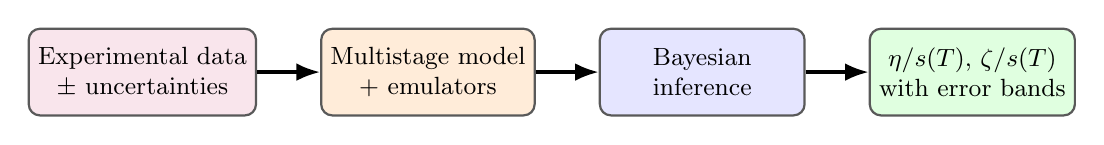
\begin{tikzpicture}[
  box/.style={rounded corners,draw=black!65,thick,minimum width=2.6cm,minimum height=1.1cm,align=center,font=\small},
  arr/.style={-{Latex[length=3mm]},very thick}
]
\node<1->[box,fill=purple!10] (data) {Experimental data\\$\pm$ uncertainties};
\node<2->[box,fill=orange!15,right=.8cm of data] (model) {Multistage model\\+ emulators};
\node<3->[box,fill=blue!10,right=.8cm of model] (bayes) {Bayesian\\inference};
\node<4->[box,fill=green!12,right=.8cm of bayes] (qgp) {$\etas(T)$, $\zetas(T)$\\with error bands};
\draw<2->[arr] (data)--(model);
\draw<3->[arr] (model)--(bayes);
\draw<4->[arr] (bayes)--(qgp);
\end{tikzpicture}
\vspace{6mm}

\raggedright
\begin{itemize}
  \item<3-> Model-to-data comparison is now a precision programme: hundreds of data points, $\sim$15--20 parameters.
  \item<4-> The headline result is not only a value of $\etas$: it is its \textbf{uncertainty}.
\end{itemize}
\vspace{3mm}
\uncover<5->{%
\begin{alertblock}{This talk}
The width of the posterior depends on an input we do not have: the correlations between experimental uncertainties.
\end{alertblock}
}
\smallcite{JETSCAPE, Phys. Rev. C 103, 054904 (2021); Bernhard, Moreland, Bass, Nature Phys. 15, 1113 (2019); Nijs et al., PRL 126, 202301 (2021)}
\end{frame}

% ------------------------------------------------------------
\begin{frame}{Where the experimental uncertainty enters}
\uncover<1->{%
\[
P(\boldsymbol{\theta}\mid D)\propto \mathcal{L}(D\mid\boldsymbol{\theta})\,P(\boldsymbol{\theta}),
\qquad
\ln\mathcal{L}=-\frac12\,\Delta y^{T}\,\Sigma^{-1}\,\Delta y-\frac12\ln\det\Sigma+\text{const}
\]
}
\uncover<2->{%
\[
\Delta y = y_{\rm exp}-y_{\rm model}(\boldsymbol{\theta}),
\qquad
\Sigma=\underbrace{\Semu(\boldsymbol{\theta})}_{\text{known: GP emulator}}
+\underbrace{\Sexp}_{\text{\alert{only partly known}}}
\]
}
\vspace{1mm}
\begin{itemize}
  \item<3-> Experiments publish $\sigma_i^{\rm stat}$ and $\sigma_i^{\rm sys}$ for each point: the \textbf{diagonal} of $\Sexp$.
  \item<4-> The off-diagonal elements $\Sexp_{ij}$ are, in general, not reported.
  \item<5-> Standard practice: $\Sexp_{ij}=\sigma_i^2\,\delta_{ij}$ \ (all points treated as independent).
\end{itemize}
\end{frame}

% ------------------------------------------------------------
\begin{frame}{Systematic uncertainties are correlated}
\begin{columns}[T,onlytextwidth]
\column{.52\textwidth}
\uncover<1->{Systematics dominate over statistics for bulk observables, and their sources are shared:}
\begin{itemize}
  \item<2-> tracking efficiency, $\pt$ extrapolation $\Rightarrow$ yields and $\mean{\pt}$ in \textbf{all centralities};
  \item<3-> centrality determination $\Rightarrow$ neighbouring bins move together;
  \item<4-> particle identification, feed-down $\Rightarrow$ across \textbf{species};
  \item<5-> non-flow subtraction $\Rightarrow$ across \textbf{harmonics} $v_n$.
\end{itemize}
\column{.45\textwidth}
\centering
\uncover<6->{%
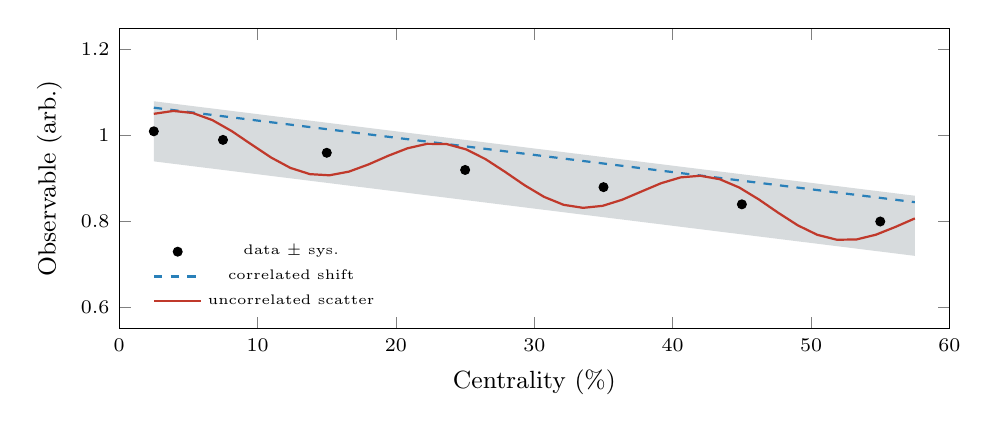
\begin{tikzpicture}
\begin{axis}[
  width=\linewidth,height=5.4cm,
  xlabel={Centrality (\%)},ylabel={Observable (arb.)},
  xmin=0,xmax=60,ymin=0.55,ymax=1.25,
  label style={font=\small},tick label style={font=\scriptsize},
  legend style={font=\tiny,draw=none,fill=none,at={(0.03,0.03)},anchor=south west}
]
\addplot[name path=up,draw=none,forget plot,domain=2.5:57.5,samples=12] {1.02-0.004*x+0.07};
\addplot[name path=dn,draw=none,forget plot,domain=2.5:57.5,samples=12] {1.02-0.004*x-0.07};
\addplot[qcdGray!60,forget plot] fill between[of=up and dn];
\addplot[only marks,mark=*,mark size=1.6pt,black] coordinates
 {(2.5,1.01) (7.5,0.99) (15,0.96) (25,0.92) (35,0.88) (45,0.84) (55,0.80)};
\addlegendentry{data $\pm$ sys.}
\addplot[qcdBlue,thick,dashed,domain=2.5:57.5,samples=2] {1.02-0.004*x+0.055};
\addlegendentry{correlated shift}
\addplot[qcdRed,thick,domain=2.5:57.5,samples=40] {1.02-0.004*x+0.055*sin(deg(x/3))};
\addlegendentry{uncorrelated scatter}
\end{axis}
\end{tikzpicture}%
}
\end{columns}
\vspace{1mm}
\uncover<7->{\small Both curves have the same diagonal $\chi^2$. Only one of them is a plausible systematic effect.}
\end{frame}

% ------------------------------------------------------------
\begin{frame}{Why it matters: how many independent measurements?}
\begin{columns}[T,onlytextwidth]
\column{.5\textwidth}
\uncover<1->{$N$ points with equal errors $\sigma$ and uniform correlation $\rho$:}
\uncover<1->{%
{\small\[
\operatorname{Var}(\bar y)=\tfrac{\sigma^2}{N}\big[1+(N-1)\rho\big]
\uncover<2->{\;\Rightarrow\; N_{\rm eff}=\frac{N}{1+(N-1)\rho}}
\]}
}
\vspace{-2mm}
\begin{itemize}
  \item<3-> Ignoring $\rho$ counts the same information $N$ times: the overall scale looks \textbf{too well known}.
  \item<4-> But the \emph{shape} across bins is constrained \textbf{more} tightly.
\end{itemize}
\column{.47\textwidth}
\centering
\uncover<2->{%
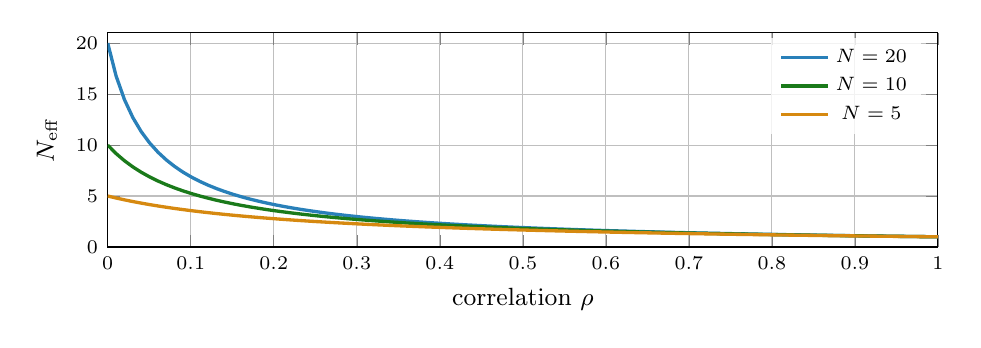
\begin{tikzpicture}
\begin{axis}[
  width=\linewidth,height=4.3cm,
  xlabel={correlation $\rho$},ylabel={$N_{\rm eff}$},
  xmin=0,xmax=1,ymin=0,ymax=21,
  grid=major,label style={font=\small},tick label style={font=\scriptsize},
  legend style={font=\scriptsize,draw=none,fill=white,fill opacity=.8,text opacity=1}
]
\addplot[qcdBlue,very thick,domain=0:1,samples=100] {20/(1+19*x)};
\addlegendentry{$N=20$}
\addplot[qcdGreen,very thick,domain=0:1,samples=100] {10/(1+9*x)};
\addlegendentry{$N=10$}
\addplot[qcdOrange,very thick,domain=0:1,samples=100] {5/(1+4*x)};
\addlegendentry{$N=5$}
\end{axis}
\end{tikzpicture}%
}
\end{columns}
\vspace{-2mm}
\uncover<5->{%
\begin{alertblock}{Not just a rescaling of error bars}
Correlations change which \emph{directions} in data space are well measured: posteriors can broaden, narrow or shift.
\end{alertblock}
}
\end{frame}

% ------------------------------------------------------------
\begin{frame}{A known warning: the viscosity posterior broadens}
\begin{columns}[T,onlytextwidth]
\column{.56\textwidth}
\centering
\uncover<1->{%
\plotorph{jetscape_fig23_viscous_posterior.pdf}{\linewidth}{5.0cm}{$\etas(T)$ and $\zetas(T)$ posteriors (Grad)\\solid: diagonal $\Sexp$ \quad dashed: correlated $\Sexp$\\(JETSCAPE, PRC 103, 054904, Fig.~23)}
}
\column{.41\textwidth}
\uncover<2->{{\Large Same data, same model.}}\\[2mm]
\uncover<3->{{\Large Different assumption about $\Sexp$.}}
\vspace{4mm}

\normalsize
\begin{itemize}
  \item<4-> A simple correlated ansatz visibly \textbf{broadens} the $\etas$ and $\zetas$ bands.
  \item<5-> The quoted uncertainty of QGP transport coefficients depends on an untested assumption.
\end{itemize}
\end{columns}
\smallcite{JETSCAPE Collaboration, Phys. Rev. C 103, 054904 (2021), App.~D}
\end{frame}

% ------------------------------------------------------------
\begin{frame}{Two simple correlation models}
\begin{columns}[T,onlytextwidth]
\column{.5\textwidth}
\uncover<1->{$\Sexp_{ij}=\rho_{ij}\,\sigma_i\,\sigma_j$ between centrality bins $c_i$, $c_j$:}
\vspace{1mm}

\uncover<2->{\textbf{Compound symmetry:} one common correlation}
\uncover<2->{%
\[
\rho_{ij}=\rho\quad(i\neq j)
\]
}
\vspace{-3mm}
\uncover<3->{\textbf{RBF:} decays with distance in centrality}
\uncover<3->{%
\[
\rho_{ij}=\exp\!\left[-\frac{(c_i-c_j)^2}{\ell^2}\right]
\]
}
\vspace{-3mm}
\begin{itemize}
  \item<4-> JETSCAPE test: RBF with $\ell=0.5$; factor $0.8$ between observables of the same group; zero between groups.
\end{itemize}
\column{.47\textwidth}
\centering
\uncover<3->{%
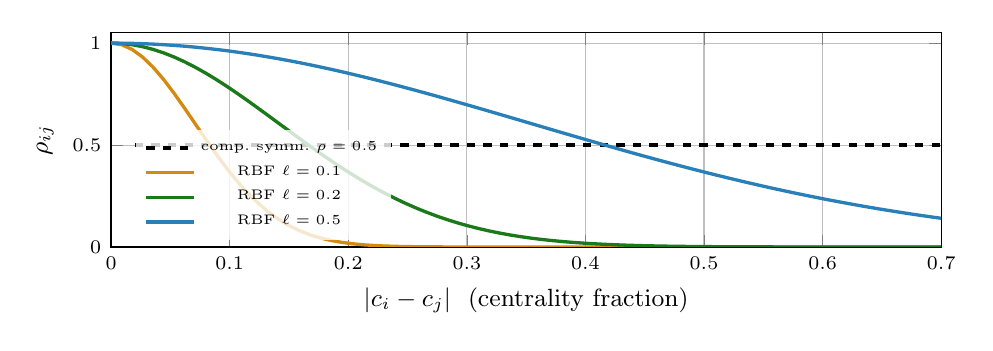
\begin{tikzpicture}
\begin{axis}[
  width=\linewidth,height=4.3cm,
  xlabel={$|c_i-c_j|$ \ (centrality fraction)},ylabel={$\rho_{ij}$},
  xmin=0,xmax=0.7,ymin=0,ymax=1.05,
  grid=major,label style={font=\small},tick label style={font=\scriptsize},
  legend style={font=\tiny,draw=none,fill=white,fill opacity=.8,text opacity=1,at={(0.03,0.03)},anchor=south west}
]
\addplot[black,very thick,dashed,domain=0.02:0.7,samples=2] {0.5};
\addlegendentry{comp.\ symm.\ $\rho=0.5$}
\addplot[qcdOrange,very thick,domain=0:0.7,samples=80] {exp(-x^2/0.01)};
\addlegendentry{RBF $\ell=0.1$}
\addplot[qcdGreen,very thick,domain=0:0.7,samples=80] {exp(-x^2/0.04)};
\addlegendentry{RBF $\ell=0.2$}
\addplot[qcdBlue,very thick,domain=0:0.7,samples=80] {exp(-x^2/0.25)};
\addlegendentry{RBF $\ell=0.5$}
\end{axis}
\end{tikzpicture}%
}
\end{columns}
\vspace{-1mm}
\uncover<5->{%
\begin{alertblock}{Both are assumptions}
Neither $\rho$ nor $\ell$ is known. How much do the conclusions depend on them?
\end{alertblock}
}
\end{frame}

% ------------------------------------------------------------
\begin{frame}{Setup}
\begin{columns}[T,onlytextwidth]
\column{.5\textwidth}
\begin{itemize}
  \item<1-> \textbf{Model:} JETSCAPE multistage hybrid, 17 parameters, Grad viscous correction.
  \item<1-> \textbf{System:} Pb--Pb at $\snn=2.76$ TeV, 110 data points (ALICE).
  \item<2-> \textbf{Emulators:} GPs on 10 principal components, validated on held-out design points.
  \item<3-> \textbf{Sampling:} parallel-tempering MCMC; identical settings and convergence checks for every $\Sexp$.
\end{itemize}
\vspace{1mm}
\TODO{confirm against the final analysis; state Nara's setup if different}
\column{.46\textwidth}
\uncover<4->{%
\small
\begin{tabular}{@{}ll@{}}
\toprule
\textbf{Run} & $\Sexp$ \\
\midrule
A & diagonal (standard) \\
B & compound symmetry, $\rho=$ \TODO{values} \\
C & RBF, $\ell=$ \TODO{values} \\
D & informed by the data (GP) \\
\bottomrule
\end{tabular}
\\[3mm]
\normalsize Only $\Sexp$ changes between runs.
}
\end{columns}
\smallcite{JETSCAPE, Phys. Rev. C 103, 054904 (2021); public emulators and data from the JETSCAPE Summer School 2021}
\end{frame}

% ------------------------------------------------------------
\begin{frame}{Result I: the viscosities depend on the assumed correlations}
\begin{columns}[T,onlytextwidth]
\column{.49\textwidth}
\centering
\uncover<1->{%
\plotorph{eta_s_posterior_runs.pdf}{\linewidth}{4.3cm}{$\etas(T)$ 90\% bands\\A diagonal, B compound symmetry, C RBF}
}
\column{.49\textwidth}
\centering
\uncover<2->{%
\plotorph{zeta_s_posterior_runs.pdf}{\linewidth}{4.3cm}{$\zetas(T)$ 90\% bands\\A diagonal, B compound symmetry, C RBF}
}
\end{columns}
\vspace{2mm}
\begin{itemize}
  \item<3-> \TODO{result: band width relative to diagonal, as a function of $T$}
  \item<4-> \TODO{result: trend with $\rho$ and with $\ell$}
\end{itemize}
\end{frame}

% ------------------------------------------------------------
\begin{frame}{Result II: the parameter posteriors shift}
\begin{columns}[T,onlytextwidth]
\column{.6\textwidth}
\centering
\uncover<1->{%
\plotorph{posterior_shift_cs_rbf.pdf}{\linewidth}{4.8cm}{Shift of each parameter posterior, in units of the diagonal-case $\sigma$\\compound symmetry and RBF vs.\ diagonal}
}
\column{.37\textwidth}
\uncover<2->{{\Large Shifts of more than $0.8\,\sigma$}}\\[1mm]
\uncover<2->{from the correlation model alone.}
\vspace{3mm}

\normalsize
\begin{itemize}
  \item<3-> Not only broader: central values move.
  \item<4-> \TODO{which parameters shift most; setup of this study}
\end{itemize}
\end{columns}
\end{frame}

% ------------------------------------------------------------
\begin{frame}{Case study: correlations do not always weaken a constraint}
\begin{columns}[T,onlytextwidth]
\column{.5\textwidth}
\centering
\uncover<1->{%
\plotorph{fig_w_short.pdf}{\linewidth}{3.2cm}{Marginal posterior of the nucleon width $w$}
}
\vspace{-1mm}
\uncover<3->{%
{\scriptsize\setlength{\tabcolsep}{3pt}
\begin{tabular}{@{}lccc@{}}
\toprule
Covariance of $U(x_T)$ & $\sigma/\sigma_{\rm orig}$ & $-2\Delta\ln L|_{w=1}$ & $w$ [fm], 90\% \\
\midrule
Original, diagonal & 1.00 & 8.1 & [0.50, 0.66] \\
Smooth in $\pt$ & 0.51 & 8.1 & [0.50, 0.65] \\
Norm.\ + tilt & 0.60 & 22.2 & [0.50, 0.59] \\
\bottomrule
\end{tabular}}
}
\column{.47\textwidth}
\uncover<1->{Scaled pion spectra $U(x_T)$ prefer $w\approx0.5$ fm; integrated observables prefer $w\approx1$ fm.}
\begin{itemize}
  \item<2-> Uncertainties of the \textbf{raw spectra} propagated through the scaling: 8 covariances.
  \item<3-> Errors shrink to 50--70\%: normalization cancels in $U$.
  \item<4-> The tension is \textbf{equal or stronger} in every case.
\end{itemize}
\vspace{1mm}
\uncover<5->{%
\begin{alertblock}{Lesson}
The effect has no fixed sign: it depends on how the observable is built.
\end{alertblock}
}
\end{columns}
\smallcite{Scaled spectra: Domingues et al., arXiv:2602.22490. ALICE Pb--Pb 2.76 TeV $\pi^+$, 0--60\%, 287 points.}
\end{frame}

% ------------------------------------------------------------
\begin{frame}{Can the data tell us? A Gaussian process on the measurements}
\begin{columns}[T,onlytextwidth]
\column{.5\textwidth}
\uncover<1->{For each observable, versus centrality $c$:}
\uncover<1->{%
\[
y_i=f(c_i)+\epsilon^{\rm stat}_i+\epsilon^{\rm unc}_i+\epsilon^{\rm cor}_i
\]
}
\vspace{-3mm}
\begin{itemize}
  \item<2-> $f$: smooth physical trend, GP prior.
  \item<3-> $\epsilon^{\rm stat}$: independent, $\sigma^{\rm stat}_i$ published.
  \item<4-> Systematic split by a fraction $\alpha$:
\end{itemize}
\uncover<4->{%
{\small\[
\Sigma^{\rm sys}_{ij}=\sigma^{\rm sys}_i\sigma^{\rm sys}_j
\Big[(1-\alpha)\,\delta_{ij}+\alpha\,e^{-(c_i-c_j)^2/\ell^2}\Big]
\]}
}
\uncover<5->{Hyperparameters $(\alpha,\ell)$ from the GP marginal likelihood.}
\column{.47\textwidth}
\centering
\uncover<2->{%
\plotorph{gp_fit_data.pdf}{\linewidth}{4.6cm}{HEPData points $\pm$ stat, sys (e.g.\ $v_2\{2\}$, $\mean{\pt}$)\\GP mean and band vs.\ centrality}
}
\end{columns}
\vspace{1mm}
\uncover<6->{\small The key signal: points scatter around a smooth curve \textbf{much less} than their systematic error bars allow.}
\end{frame}

% ------------------------------------------------------------
\begin{frame}{First step: what correlation do the data support?}
\begin{columns}[T,onlytextwidth]
\column{.49\textwidth}
\centering
\uncover<1->{%
\plotorph{pull_distribution.pdf}{\linewidth}{4.2cm}{Pulls of HEPData points around the smooth GP fit\\compared with $\mathcal{N}(0,1)$}
}
\column{.49\textwidth}
\centering
\uncover<2->{%
\plotorph{alpha_per_group.pdf}{\linewidth}{4.2cm}{Inferred correlated fraction $\alpha$\\per observable group}
}
\end{columns}
\vspace{2mm}
\begin{itemize}
  \item<1-> If errors were independent, pulls would follow $\mathcal{N}(0,1)$. \TODO{result: observed width}
  \item<2-> \TODO{result: $\alpha$ per group; run D viscosities vs.\ runs A--C}
  \item<3-> The long-range length $\ell$ is degenerate with the physical trend: it still needs a prior.
\end{itemize}
\end{frame}

% ------------------------------------------------------------
\begin{frame}{Outlook}
\begin{columns}[T,onlytextwidth]
\column{.49\textwidth}
\uncover<1->{%
\begin{block}{Next steps}
\begin{itemize}
  \item Propagate raw-spectra uncertainties to all integrated observables (yields, $\mean{\pt}$).
  \item Few physical modes (normalization, tilt) as nuisance parameters, marginalized.
  \item Neural simulation-based inference with correlations sampled from a prior.
  \item Closure and coverage tests.
\end{itemize}
\end{block}}
\column{.49\textwidth}
\uncover<2->{%
\begin{block}{What would help most from experiments}
\begin{itemize}
  \item \textbf{Best:} covariance matrices across centrality bins and observables (HEPData).
  \item \textbf{Very useful:} systematics split by source, flagged correlated or uncorrelated.
  \item \textbf{Minimum:} guidance for priors on correlation length and strength.
\end{itemize}
\end{block}}
\end{columns}
\vspace{2mm}
\uncover<3->{%
\begin{alertblock}{Why now}
As statistical and emulator errors shrink, the unknown off-diagonal terms become a leading uncertainty in QGP property extraction.
\end{alertblock}
}
\end{frame}

% ------------------------------------------------------------
\begin{frame}{Take-home messages}
\begin{enumerate}
  \item<1-> \textbf{An unverified assumption:} Bayesian analyses of heavy-ion data treat experimental uncertainties as uncorrelated, although systematics dominate and are correlated.
  \item<2-> \textbf{It changes the answer:} simple correlation models (compound symmetry, RBF) shift parameter posteriors by more than $0.8\,\sigma$ and change the uncertainty of $\etas(T)$ and $\zetas(T)$.
  \item<3-> \textbf{No fixed sign:} for the scaled spectra, consistent correlated uncertainties make the constraint on the nucleon width equal or stronger.
  \item<4-> \textbf{The data carry information:} a Gaussian process on the published points constrains the correlated fraction. \TODO{one-line result}
  \item<5-> \textbf{A request:} published covariance matrices, or systematics by source.
\end{enumerate}
\vspace{4mm}
\centering
\uncover<6->{{\Large\bfseries Thank you!}}
\end{frame}

% ============================================================
% BACKUP
% ============================================================
\appendix
\section{Backup}

\begin{frame}{Backup: structure of the covariance matrix}
\begin{columns}[c,onlytextwidth]
\column{.46\textwidth}
\centering
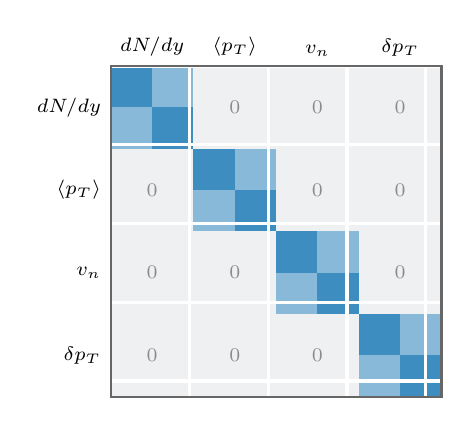
\begin{tikzpicture}[x=1.05cm,y=1.05cm,font=\scriptsize]
% 4 groups; group k occupies [k-1,k] on both axes (y downwards)
\foreach \i in {0,1,2,3}{
  \foreach \j in {0,1,2,3}{
    \ifnum\i=\j
      \fill[qcdBlue!55] (\i,-\j) rectangle ++(1,-1);
    \else
      \fill[qcdGray!25] (\i,-\j) rectangle ++(1,-1);
      \node[text=black!45] at (\i+.5,-\j-.5) {$0$};
    \fi
  }
}
% inside each diagonal block: same-observable sub-blocks darker
\foreach \k in {0,1,2,3}{
  \fill[qcdBlue!90] (\k,-\k) rectangle ++(.5,-.5);
  \fill[qcdBlue!90] (\k+.5,-\k-.5) rectangle ++(.5,-.5);
}
\draw[white,very thick] (0,0) grid (4,-4);
\draw[black!60,thick] (0,0) rectangle (4,-4);
\node[above] at (.5,0) {$dN/dy$};
\node[above] at (1.5,0) {$\mean{\pt}$};
\node[above] at (2.5,0) {$v_n$};
\node[above] at (3.5,0) {$\delta\pt$};
\node[left] at (0,-.5) {$dN/dy$};
\node[left] at (0,-1.5) {$\mean{\pt}$};
\node[left] at (0,-2.5) {$v_n$};
\node[left] at (0,-3.5) {$\delta\pt$};
\end{tikzpicture}
\column{.5\textwidth}
\begin{itemize}
  \item<1-> {\color{qcdBlue!90!black}\textbf{Dark:}} same observable, different centralities: $\rho(\Delta c)$.
  \item<2-> {\color{qcdBlue!60!black}\textbf{Light:}} different observables in the same group (e.g.\ $\pi$ and $K$ yields, $v_2$ and $v_3$): $\rho_0\,\rho(\Delta c)$.
  \item<3-> {\color{black!50}\textbf{Grey:}} different groups, uncorrelated.
\end{itemize}
\vspace{3mm}
\uncover<4->{Two numbers control everything:}
\uncover<4->{%
\[
\ell\ (\text{length}),\quad \rho_0\ (\text{intra-group strength})
\]
}
\uncover<5->{\small The matrix stays positive semi-definite for any $\ell>0$, $0\le\rho_0\le1$.}
\end{columns}
\end{frame}

% ------------------------------------------------------------
\begin{frame}{Backup: what the data can and cannot tell us}
\begin{columns}[T,onlytextwidth]
\column{.49\textwidth}
\uncover<1->{%
\begin{block}{Constrained}
\begin{itemize}
  \item The \textbf{uncorrelated} fraction $1-\alpha$: bounded by the bin-to-bin scatter.
  \item Short-range correlation between neighbouring bins.
\end{itemize}
\end{block}}
\uncover<3->{%
\centering
\plotorph{pull_distribution.pdf}{.9\linewidth}{2.6cm}{Pulls around the smooth fit vs.\ $\mathcal{N}(0,1)$}
}
\column{.49\textwidth}
\uncover<2->{%
\begin{block}{Not constrained by one data set}
\begin{itemize}
  \item A coherent shift of all bins looks like a different trend $f$.
  \item So the long-range $\ell$ is degenerate with the physics: it needs a prior.
\end{itemize}
\end{block}}
\uncover<4->{%
\textbf{Extra handles}
\begin{itemize}
  \item published uncertainties of \textbf{ratios} (species, energies, harmonics);
  \item the same observable from \textbf{different experiments};
  \item systematics listed by source on HEPData.
\end{itemize}}
\end{columns}
\smallcite{Ratio: $\sigma_R^2/R^2=\sigma_1^2/y_1^2+\sigma_2^2/y_2^2-2\rho\,\sigma_1\sigma_2/(y_1y_2)$ gives $\rho$ directly.}
\end{frame}

% ------------------------------------------------------------
\begin{frame}{Backup: scaled spectra, all alternative covariances}
\centering\scriptsize
\setlength{\tabcolsep}{4pt}
\begin{tabular}{@{}lcccccc@{}}
\toprule
 & $\sigma/\sigma_{\rm orig}$ & $\chi^2_{\rm ML}$ & $-2\Delta\ln L$ & median $w$ & 90\% interval & $P(w_{\rm sp}\ge w_{\rm int})$ \\
 & & (287 pts) & at $w=1$ & [fm] & [fm] & \\
\midrule
\emph{Integrated observables} & --- & --- & --- & 1.00 & [0.81, 1.17] & --- \\
\midrule
\textbf{Original: diagonal} & \textbf{1.00} & \textbf{26} & \textbf{8.1} & \textbf{0.54} & \textbf{[0.50, 0.66]} & \textbf{0.0013} \\
\midrule
(a) original budget, corr.\ modes & 1.06 & 43 & 10.0 & 0.53 & [0.50, 0.64] & 0.0010 \\
(b) uncorrelated, $\rho_c=0$ & 0.72 & 450 & 9.2 & 0.54 & [0.50, 0.65] & 0.0014 \\
(c) smooth, $\ell=1$, $\rho_c=0$ & 0.51 & 126 & 8.1 & 0.53 & [0.50, 0.65] & 0.0014 \\
(d) smooth, $\ell=1$, $\rho_c=1$ & 0.51 & 837 & 16.8 & 0.52 & [0.50, 0.60] & 0.0005 \\
(e) smooth, $\ell=0.3$, $\rho_c=1$ & 0.64 & 760 & 23.1 & 0.52 & [0.50, 0.60] & 0.0004 \\
(f) coherent, $\rho_c=1$ & 0.48 & 994 & 20.1 & 0.52 & [0.50, 0.60] & 0.0005 \\
(g) norm.\ + tilt, $\rho_c=0$ & 0.54 & 190 & 12.1 & 0.52 & [0.50, 0.61] & 0.0006 \\
(h) norm.\ + tilt, $\rho_c=1$ & 0.60 & 664 & 22.2 & 0.52 & [0.50, 0.59] & 0.0004 \\
\bottomrule
\end{tabular}
\vspace{2mm}

\raggedright\small
\begin{itemize}
  \item $\rho_c$: correlation of the correlated part between centrality classes. Posteriors are bounded below by the prior edge $w=0.5$ fm.
  \item With the original errors $\chi^2_{\rm ML}/287=0.09$: a sign that they are inflated.
  \item Caveats: emulator unchanged and used in extrapolation; one chain per alternative, $w$ stable along each.
\end{itemize}
\end{frame}

% ------------------------------------------------------------
\begin{frame}{Backup: propagating uncertainties to the scaled spectra}
With $U(x_T)=(\mean{\pt}/N)\,\dd N/\dd\pt$ on a fixed $x_T$ grid, to linear order:
\[
\delta U_i = U_i\,\frac{\delta y_i}{y_i} - U_i\,\frac{\delta N}{N}
+ \big(U_i + x_iU'_i\big)\frac{\delta\mean{\pt}}{\mean{\pt}},
\]
where $\delta N$ and $\delta\mean{\pt}$ follow from the same fluctuations $\delta y_j$ of the measured spectrum, plus the low-$\pt$ extrapolation uncertainties.
\begin{itemize}
  \item A common normalization change cancels in $U$, apart from the extrapolated part of the yield.
  \item The last term is the horizontal shift of the points when $\mean{\pt}$ changes.
  \item A non-linear Monte Carlo agrees with the linear propagation to 1--3\%.
\end{itemize}
\end{frame}

% ------------------------------------------------------------
\begin{frame}{Backup: correlation matrices}
\begin{columns}[T,onlytextwidth]
\column{.49\textwidth}
\centering
\uncover<1->{%
\plotorph{corr_matrix_ansatz.pdf}{\linewidth}{4.5cm}{Correlation matrix, 110 $\times$ 110\\ansatz ($\ell=0.5$, $\rho_0=0.8$)}
}
\column{.49\textwidth}
\centering
\uncover<2->{%
\plotorph{corr_matrix_gp.pdf}{\linewidth}{4.5cm}{Correlation matrix, 110 $\times$ 110\\GP-learned from HEPData}
}
\end{columns}
\vspace{2mm}
\begin{itemize}
  \item<3-> \TODO{result: inferred $\alpha$ and $\ell$ per observable group; where they differ from the ansatz}
\end{itemize}
\end{frame}

% ------------------------------------------------------------
\begin{frame}{Backup: which parameters are most sensitive?}
\begin{columns}[T,onlytextwidth]
\column{.6\textwidth}
\centering
\uncover<1->{%
\plotorph{parameter_widths_runs.pdf}{\linewidth}{4.8cm}{90\% interval of each of the 17 parameters\\runs A--D (normalized to prior width)}
}
\column{.37\textwidth}
\uncover<2->{{\Large Not all parameters react the same way.}}
\vspace{3mm}

\normalsize
\begin{itemize}
  \item<3-> Parameters fixed by \textbf{overall scales} lose constraint.
  \item<4-> Parameters fixed by \textbf{centrality dependence} can gain.
  \item<5-> \TODO{result: confirm with the posteriors}
\end{itemize}
\end{columns}
\end{frame}

% ------------------------------------------------------------
\begin{frame}{Backup: closure tests}
\begin{columns}[T,onlytextwidth]
\column{.5\textwidth}
\centering
\uncover<2->{%
\plotorph{closure_coverage.pdf}{\linewidth}{4.4cm}{Closure: true vs.\ inferred $\etas$, $\zetas$\\pseudo-data with correlated noise, analysed with\\(a) diagonal \ (b) GP-learned $\Sexp$}
}
\column{.47\textwidth}
\uncover<1->{Pseudo-data from the model at known $\boldsymbol{\theta}_{\rm true}$, with noise drawn from a \textbf{known correlated} $\Sexp$.}
\vspace{3mm}

\begin{itemize}
  \item<2-> Does the GP recover the injected $(\alpha,\ell)$?
  \item<3-> Diagonal analysis: does the 90\% band contain the truth 90\% of the time?
  \item<4-> GP-learned analysis: is coverage restored?
  \item<5-> \TODO{result}
\end{itemize}
\end{columns}
\end{frame}

% ------------------------------------------------------------
\begin{frame}{Backup: full likelihood}
\[
\ln \mathcal{L}(\boldsymbol{\theta},\ell,\rho_0) =
-\frac12 \Delta y^T\Sigma^{-1}\Delta y
-\frac12\ln\det\Sigma-\frac{n}{2}\ln(2\pi),
\]
\[
\Delta y=y_{\rm exp}-y_{\rm emu}(\boldsymbol{\theta}),\qquad
\Sigma=\Sexp(\ell,\rho_0)+\Semu(\boldsymbol{\theta}).
\]
\begin{itemize}
  \item With fixed $\Sexp$ the determinant only matters through $\Semu(\boldsymbol{\theta})$.
  \item With free $(\ell,\rho_0)$ it acts as an Occam penalty: stronger correlations shrink $\det\Sigma$ but make deviations orthogonal to the correlated direction more costly.
\end{itemize}
\end{frame}

% ------------------------------------------------------------
\begin{frame}{Backup: statistical versus systematic parts}
A more careful decomposition keeps the statistical part diagonal:
\[
\Sexp_{ij}=\big(\sigma^{\rm stat}_i\big)^2\delta_{ij}
+\rho_{ij}\,\sigma^{\rm sys}_i\,\sigma^{\rm sys}_j .
\]
\begin{itemize}
  \item Statistical errors of different bins are independent (different events).
  \item Exception: observables built from the same events (e.g.\ $v_2\{2\}$ and $v_3\{2\}$ in one centrality bin) have correlated statistical errors too.
  \item \TODO{state which convention is used in the results}
\end{itemize}
\end{frame}

% ------------------------------------------------------------
\begin{frame}{Backup: positive semi-definiteness}
The ansatz is a product of valid kernels:
\[
\rho_{(a,i),(b,j)}=
\underbrace{R_{ab}}_{\text{observables}}\;
\underbrace{\exp\!\left[-\frac{(c_i-c_j)^2}{\ell^2}\right]}_{\text{centrality}},
\qquad
R_{ab}=\begin{cases}1 & a=b\\ \rho_0 & a\neq b,\ \text{same group}\\ 0 & \text{different groups}\end{cases}
\]
\begin{itemize}
  \item The squared-exponential kernel is positive semi-definite for any $\ell>0$.
  \item $R$ is block diagonal with eigenvalues $1-\rho_0$ and $1+(m-1)\rho_0$ ($m$ observables in the group): positive for $0\le\rho_0<1$.
  \item Their product (Schur product theorem) is positive semi-definite.
  \item In practice: large $\ell$ makes $\Sexp$ nearly singular; $\Semu$ and $\sigma^{\rm stat}$ regularize it.
\end{itemize}
\end{frame}

% ------------------------------------------------------------
\begin{frame}{Backup: two-point intuition}
Two measurements with errors $\sigma$ and correlation $\rho$. In the rotated variables
\[
y_\pm=\frac{y_1\pm y_2}{\sqrt2}:\qquad
\operatorname{Var}(y_+)=\sigma^2(1+\rho),\qquad
\operatorname{Var}(y_-)=\sigma^2(1-\rho).
\]
\begin{itemize}
  \item The \textbf{sum} (overall level) is known less precisely.
  \item The \textbf{difference} (slope, centrality dependence) is known more precisely.
  \item A parameter constrained by the level broadens; one constrained by the slope narrows.
\end{itemize}
\end{frame}

% ------------------------------------------------------------
\begin{frame}{Backup: alternative correlation models}
\begin{itemize}
  \item \textbf{Fully correlated normalization:} one nuisance shift per observable, $y\to(1+\epsilon)\,y$, $\epsilon\sim\mathcal{N}(0,\sigma_{\rm norm})$. Equivalent to a rank-one term in $\Sexp$.
  \item \textbf{Exponential kernel:} $\rho_{ij}=\exp(-|c_i-c_j|/\ell)$, rougher than the Gaussian form.
  \item \textbf{Separate $\ell$ per group:} flow systematics need not share the length scale of yields.
  \item \textbf{Cross-group correlations:} e.g.\ yields and $\mean{\pt}$ share tracking efficiency and $\pt$ extrapolation.
\end{itemize}
\vspace{2mm}
\TODO{keep only the variants actually tested; add comparison plot}

\plotorph{kernel_comparison.pdf}{.5\linewidth}{2.4cm}{Posterior comparison between kernels}
\end{frame}

% ------------------------------------------------------------
\begin{frame}{Backup: prior and posterior predictive}
\begin{columns}[T,onlytextwidth]
\column{.49\textwidth}
\centering
\plotorph{posterior_predictive_diag.pdf}{\linewidth}{4.6cm}{Observables: posterior predictive, diagonal $\Sexp$}
\column{.49\textwidth}
\centering
\plotorph{posterior_predictive_corr.pdf}{\linewidth}{4.6cm}{Observables: posterior predictive, marginalized $\Sexp$}
\end{columns}
\vspace{2mm}
\small With correlated errors a good fit may sit coherently above or below the points: judge it with the full $\chi^2$, not by eye.
\end{frame}

% ------------------------------------------------------------
\begin{frame}{Backup: full parameter posterior}
\centering
\plotorph{corner_diag_vs_corr.pdf}{.62\linewidth}{6.0cm}{Corner plot of all model parameters\\diagonal (blue) vs.\ correlated/marginalized (orange)}
\end{frame}

\end{document}
